%%%%%%%%%%%%%%%%%%%%%%%%%%%%%%%%%%%%%%%%%
%
% (c) 2022 by Jennifer Laaser
%
% This work is licensed under the Creative Commons Attribution-NonCommercial-ShareAlike 4.0 International License. To view a copy of this license, visit http://creativecommons.org/licenses/by-nc-sa/4.0/ or send a letter to Creative Commons, PO Box 1866, Mountain View, CA 94042, USA.
%
% The current source for these materials is accessible on Github: https://github.com/jlaaser/pogil-polymers
%
%%%%%%%%%%%%%%%%%%%%%%%%%%%%%%%%%%%%%%%%%

\renewcommand{\figpath}{content/polymchem/livingpolyms/ionic-polyms/figs}
\renewcommand{\labelbase}{ionic-polyms}

\begin{activity}{Ionic Polymerizations}

\begin{instructornotes}
	This activity introduces students to concepts related to anionic and cationic polymerizations.
	
	After completing this activity, students will be able to:
	\begin{enumerate}
		\item \dots
	\end{enumerate}
	
	\subsection*{Activity summary:}
	\begin{itemize}
		\item \textbf{Activity type:} Learning Cycle
		\item \textbf{Content goals:} Ionic Polymerizations
		\item \textbf{Process goals:} %https://pogil.org/uploads/attachments/cj54b5yts006cklx4hh758htf-process-skills-official-pogil-list-2015-original.pdf
			\begin{itemize}
				\item Reading and interpreting reaction mechanisms
				\item \dots
				\item Oral and written communication of reasoning
			\end{itemize}
		\item \textbf{Duration:} 45 minutes, including class discussion
		\item \textbf{Instructor preparation required:} none beyond knowledge of relevant content
		\item \textbf{Related textbook chapters:}
			\begin{itemize}
				\item \emph{Polymer Chemistry} (Hiemenz \& Lodge): section 4.3
			\end{itemize}
		%\item \textbf{Facilitation notes:}
		%	\begin{itemize}
		%		\item \dots
		%	\end{itemize}
	\end{itemize}
	
\end{instructornotes}


\begin{model}[Anionic Polymerization]
	\label{\labelbase:mdl:anionic}

	Anionic polymerization is a popular method for producing polymers with well-controlled molecular weights.  The initiation and propagation steps of the anionic polymerization of a vinyl-type monomer are outlined below:
	
	\centerline{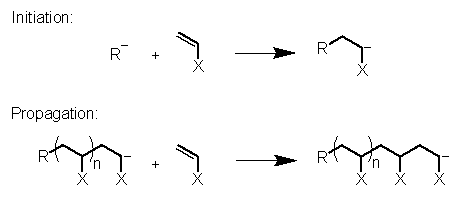
\includegraphics[width=0.7\textwidth]{\figpath/MODEL1_mainscheme}}
	
\end{model}


\begin{ctqs}

	%\question What is the reactive species on the initiator and chain ends in this type of polymerization?
	
	\question Which reagent determines the number of polymer chains formed in this reaction?
	
		\begin{solution}[0.5in]
		\end{solution}
	
	\question If the reaction proceeds to 100\% conversion (i.e. 100\% of the monomer is used up in the reaction), how would you expect the degree of polymerization of the resulting polymer to be related to the initiator and monomer concentrations, $[I]_0$ and $[M]_0$?
	
		\begin{solution}[0.5in]
		\end{solution}
	
	\question One initiator that can be used in anionic polymerization is \emph{sec}-butyllithium, shown below:
	 \label{\labelbase:ctq:ps-anionic-prop}
	
	\centerline{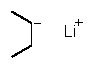
\includegraphics[width=0.15\textwidth]{\figpath/MODEL1_secBuLi}}
	 	
	 	Draw the structure of the propagating chain that would be formed if this reagent were used to initiate anionic polymerization of polystyrene.
	 	
	 	\emph{Note: For the purposes of this question, you can assume that the lithium ion does not participate in the reaction in any way.}
	
		\begin{solution}[1in]
		\end{solution}
	
	\question Suppose two propagating anions encounter each other in solution, as shown below:
	
	\centerline{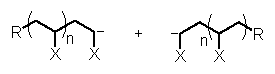
\includegraphics[width=0.4\textwidth]{\figpath/MODEL1_anionterm}}
	
		Do you expect these two anions to be able to react to form inactive (``dead'') polymer chains?  Explain your group's reasoning in 1-2 complete sentences.
	
		\begin{solution}[1.25in]
		\end{solution}
	
	\question On the basis of your answer to the previous question, do you expect anionic polymerization to meet the criteria required for an ideal, living polymerization?  Explain your group's reasoning in 2-3 complete sentences.
	
		\begin{solution}[1.25in]
		\end{solution}

\end{ctqs}

\begin{infobox}

	If the propagating anion encounters a molecule with a labile proton, it will typically be favorable for it to abstract that proton, as shown below:
	
	\centerline{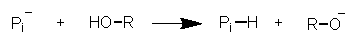
\includegraphics[width=0.6\textwidth]{\figpath/MODEL1_labileproton}}
	
\end{infobox}

\begin{ctqs}
	
	%\question Briefly describe what you would expect to happen to the propagating species in an anionic polymerization if the reaction mixture contained a small amount of water.  In this case, would the reaction still be an ideal, living polymerization?
	
	\question Why might we say that the presence of a species with a labile proton terminates the propagating anionic chain?  Explain your group's reasoning in 1-2 complete sentences.
	
		\begin{solution}[1.25in]
		\end{solution}
	
	\question If your reaction mixture contained a small amount of water, would you still expect the reaction to qualify as an ideal, living polymerization?  Why or why not?
	
		\begin{solution}[1.25in]
		\end{solution}
	
	\question Based on your answer to the previous question, explain, in 1-2 complete sentences, why it is typically critical that the solvent and monomers used in anionic polymerizations are \emph{rigorously} dried before use.
	
		\begin{solution}[1.25in]
		\end{solution}
	
\end{ctqs}

\begin{infobox}

	While \emph{unintentional} introduction of hydroxyl-containing species causes problems with anionic polymerization, \emph{intentional} introduction of a hydroxyl-containing species at the end of the reaction can be a useful way to terminate the polymer in a well-controlled way.  For example, anionic polymerizations are often terminated by addition of a small amount of methanol.

\end{infobox}

\begin{ctqs}

	\question Predict the structure of the polymer that you would obtain if you terminated the propagating anionic chain you drew in CTQ \ref{\labelbase:ctq:ps-anionic-prop} by adding methanol at the end of the reaction.
	
		\begin{solution}[2in]
		\end{solution}

	%\question introduce idea that other types of monomers can also go by anionic -> show propagation step of ethylene oxide (mention that it is a ring-opening polym, which we we will explore more later) and ask them to predict product when RO- polyms ethylene oxide w/methanol to terminate
		
\end{ctqs}


\clearpage
\begin{model}[Polymerization of Ethylene Oxide]
	\label{\labelbase:mdl:anionicEO}

	Although anionic polymerization is shown using a vinyl type monomer in Model \ref{\labelbase:mdl:anionic}, above, it can be used to polymerize a number of other types of monomers, as well.
	
	One common monomer polymerized by anionic polymerization is ethylene oxide.  Polymerization of this monomer proceeds as shown below:
	
	\centerline{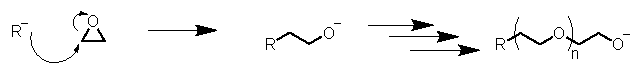
\includegraphics[width=0.9\textwidth]{\figpath/MODEL2_EOprop}}

\end{model}

\begin{ctqs}
	
	\question Why do you think polymerization of ethylene oxide is referred to as a ``ring-opening'' polymerization?  Explain your group's reasoning in 1-2 complete sentences.
	
		\begin{solution}[1in]
		\end{solution}
	
	\question Predict the structure of the polymer that you would obtain if you used the propagating chain from CTQ \ref{\labelbase:ctq:ps-anionic-prop} as the initiator for polymerization of ethylene oxide, and if you terminated the reaction with methanol after all of the ethylene oxide was used up.
	
		\begin{solution}[1.5in]
		\end{solution}
	
	\question Propose a complete name for the polymer you drew in the previous question.  Make sure the name you propose clearly specifies the identity (or identities) of the constituent polymers, whether the polymer is a homopolymer, copolymer, or terpolymer, and what its general chain architecture and sequence type are. 
	
		\begin{solution}[1.5in]
		\end{solution}
		
	\question Critique or defend the following statement in 2-3 complete sentences:
	
		\emph{``The living nature of anionic polymerizations makes them a useful way to synthesize block copolymers.''}
		
		\begin{solution}[1.5in]
		\end{solution}
	
\end{ctqs}


%\begin{exercises}

%	\exercise exercise re. the cation

%	\exercise question re. expected behavior of a PS-b-PEO block copolymer if dissolved in water, in limit that PS length > EO, PS = EO, PS < EO
	
%\end{exercises}


%\begin{problems}
%
%	\problem First exercise
%	\problem Second exercise
%	
%\end{problems}


	
\end{activity}